% ============================================================
%  CHAPTER 3: SYSTEM DESIGN AND ARCHITECTURE
% ============================================================

\chapter{SYSTEM DESIGN AND ARCHITECTURE}
\label{chap:system_design}
\label{chap:security_analysis}
\label{chap:android_ui}

\section{System Architecture Overview and Network Topology}
\label{sec:overall_architecture}

QuantumSafe VPN implements an end-to-end, post-quantum secure tunneling architecture between an unprivileged Android client and a hardened Linux security gateway. As illustrated in Figure~\ref{fig:deployment_topology}, the system partitions responsibilities across three discrete layers:
\begin{enumerate}
    \item \textbf{Android Client Layer:} Captures user-space IP traffic through the \texttt{android.net.}\allowbreak\texttt{VpnService} API, negotiates ephemeral lattice keys via pure-Kotlin PQC primitives, and encapsulates raw datagrams inside authenticated frames.
    \item \textbf{Untrusted WAN Transit Layer:} Transports length-prefixed, ciphertext frames over TCP port 7000.
    \item \textbf{Linux Gateway Layer:} Authenticates incoming sessions via ML-DSA-65 signatures, decapsulates ML-KEM-1024 shared secrets, leases private virtual IPv4 addresses, and performs kernel-level IP forwarding and Network Address Translation (NAT).
\end{enumerate}

\begin{figure}[htbp]
  \centering
  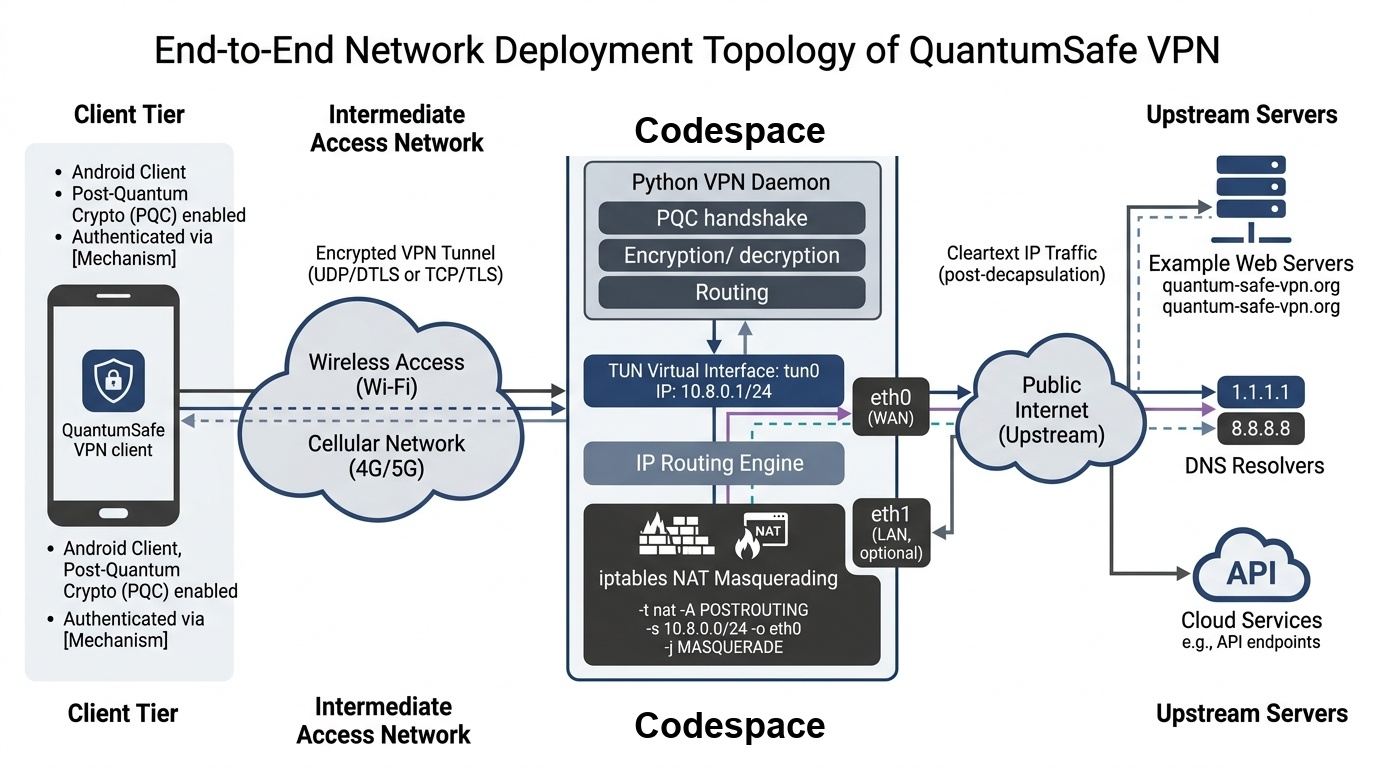
\includegraphics[width=0.88\linewidth,height=0.30\textheight,keepaspectratio]{figures/deployment_topology_concept.jpg}
  \caption[End-to-End Network Deployment Topology]{End-to-End Network Deployment Topology: This figure illustrates the three-tier system architecture and secure component placement across the Android client, WAN transit, and Linux gateway.}
  \label{fig:deployment_topology}
\end{figure}

\section{Binary Wire Framing Specification}
\label{sec:wire_framing_design}

Every frame transmitted over the TCP stream begins with a mandatory 4-byte big-endian length prefix, followed by the authenticated payload structure illustrated in Figure~\ref{fig:tikz_packet_framing}:
\begin{equation}
\label{eq:wire_framing_equation}
\begin{split}
\text{Wire Frame} = {} & \underbrace{[\text{Length} : 4\text{B}]}_{\text{Framing}} \parallel \underbrace{[IV : 12\text{B}]}_{\text{Nonce}} \parallel \underbrace{[\text{Auth Tag} : 16\text{B}]}_{\text{Galois MAC}} \\
& \parallel \underbrace{\text{AES-GCM}_{\text{Key}}\Big([\text{Seq} : 8\text{B}] \parallel [\text{Raw IPv4 Datagram}]\Big)}_{\text{Encrypted Payload}}
\end{split}
\end{equation}

\begin{figure}[htbp]
  \centering
  \begin{tikzpicture}[
    scale=0.80, every node/.style={transform shape},
    field/.style={draw=darkcharcoal, thick, fill=white, minimum height=1.1cm, align=center, font=\footnotesize\bfseries},
    headerfield/.style={field, fill=blue!10},
    ivfield/.style={field, fill=teal!10},
    seqfield/.style={field, fill=yellow!15},
    payloadfield/.style={field, fill=vpnblue!15},
    tagfield/.style={field, fill=red!10}
  ]
    \node[headerfield, minimum width=2.2cm] (len) at (0, 0) {Length\\(4B)};
    \node[ivfield, minimum width=2.4cm] (iv) at (2.3, 0) {GCM Nonce\\(12B)};
    \node[seqfield, minimum width=2.4cm] (seq) at (4.7, 0) {Monotonic Seq\\(8B)};
    \node[payloadfield, minimum width=4.5cm] (data) at (8.2, 0) {Raw IPv4 Datagram\\(Up to MTU)};
    \node[tagfield, minimum width=2.4cm] (tag) at (11.7, 0) {Auth Tag\\(16B)};

    \draw[thick, decorate, decoration={brace, amplitude=5pt, mirror}] (-1.1, -0.8) -- (12.9, -0.8)
      node[midway, yshift=-0.45cm, font=\footnotesize\bfseries] {Total Wire Frame Transmitted over TCP Stream};

    \draw[thick, decorate, decoration={brace, amplitude=5pt}] (3.5, 0.8) -- (10.5, 0.8)
      node[midway, yshift=0.45cm, font=\scriptsize\bfseries, text=vpnblue] {Encrypted \& Authenticated via AES-256-GCM};
  \end{tikzpicture}
  \caption[Binary Wire Framing Format]{Binary Wire Framing Format: This figure illustrates the byte-level frame layout including 4-byte length prefix, 12-byte GCM nonce, 8-byte sequence counter, encrypted IPv4 datagram, and 16-byte Galois MAC authentication tag.}
  \label{fig:tikz_packet_framing}
\end{figure}

\section{Cryptographic Handshake Protocol Sequence}
\label{sec:handshake_sequence}

Figure~\ref{fig:tikz_handshake_seq} details the four-stage post-quantum cryptographic handshake establishing the tunnel session:
\begin{enumerate}
    \item \textbf{Stage 1 (Server Identity):} The gateway transmits its static ML-DSA-65 public key (1,952 bytes).
    \item \textbf{Stage 2 (Client Ephemeral KEM):} The client generates an ephemeral ML-KEM-1024 keypair and dispatches its public key (1,568 bytes).
    \item \textbf{Stage 3 (Encapsulation and Signature):} The gateway encapsulates a 32-byte shared secret, signs the session transcript using ML-DSA-65 (3,309 bytes signature), and appends the JSON network lease configuration.
    \item \textbf{Stage 4 (Key Derivation):} Both endpoints independently derive an identical 256-bit symmetric key via HKDF-SHA256 (RFC 5869) and configure their local TUN routing adapters.
\end{enumerate}

\begin{figure}[htbp]
  \centering
  \begin{tikzpicture}[
    scale=0.80, every node/.style={transform shape},
    lifeline/.style={thick, dashed, draw=mutedgrey},
    nodeblock/.style={draw=darkcharcoal, thick, fill=white, rounded corners=3pt, minimum width=2.8cm, minimum height=0.9cm, align=center, font=\footnotesize\bfseries},
    msg/.style={thick, ->, >=stealth, font=\scriptsize}
  ]
    \node[nodeblock] (ui) at (0, 0) {Android UI\\(Compose)};
    \node[nodeblock] (vpn) at (3.5, 0) {VpnService\\(Worker Threads)};
    \node[nodeblock] (pqc) at (7.0, 0) {PQC Engine\\(ML-KEM/DSA)};
    \node[nodeblock] (srv) at (11.0, 0) {VPN Server\\(tunnel\_server.py)};

    \draw[lifeline] (ui) -- ++(0, -8.5);
    \draw[lifeline] (vpn) -- ++(0, -8.5);
    \draw[lifeline] (pqc) -- ++(0, -8.5);
    \draw[lifeline] (srv) -- ++(0, -8.5);

    \draw[msg] (0, -0.8) -- node[above] {User taps Connect} (3.5, -0.8);
    \draw[msg] (3.5, -1.4) -- node[above] {protect(socket)} (3.5, -1.8);
    \draw[msg] (3.5, -2.3) -- node[above] {TCP Connect (Port 7000)} (11.0, -2.3);

    \draw[msg] (11.0, -3.0) -- node[above] {Stage 1: Server ML-DSA-65 PK (1952B)} (3.5, -3.0);
    \draw[msg] (3.5, -3.5) -- node[above] {Generate Ephemeral ML-KEM} (7.0, -3.5);
    \draw[msg] (7.0, -4.2) -- node[above] {Stage 2: Client ML-KEM-1024 PK (1568B)} (11.0, -4.2);

    \draw[msg] (11.0, -4.9) -- node[above] {Encapsulate \& Sign Transcript} (11.0, -5.3);
    \draw[msg] (11.0, -5.9) -- node[above] {Stage 3: Ciphertext (1568B) + Sig (3309B) + Config} (3.5, -5.9);

    \draw[msg] (3.5, -6.5) -- node[above] {Verify Sig \& Decapsulate Secret} (7.0, -6.5);
    \draw[msg] (7.0, -7.2) -- node[above] {Derive Session Key (HKDF-SHA256)} (7.0, -7.6);
    \draw[msg] (3.5, -8.0) -- node[above] {State: CONNECTED} (0, -8.0);
  \end{tikzpicture}
  \caption[UML Sequence Diagram: 4-Stage Post-Quantum Handshake]{UML Sequence Diagram: This figure illustrates the 4-stage post-quantum cryptographic handshake protocol execution between the Android Compose UI, worker threads, PQC engine, and the remote Linux server daemon.}
  \label{fig:tikz_handshake_seq}
\end{figure}

\section{Mathematical Formulations of Security Goals}
\label{sec:math_formulations_security}
\label{sec:security_objectives}

The cryptographic architecture of QuantumSafe VPN is engineered to provide uncompromising mathematical and protocol-level guarantees:
\begin{enumerate}
    \item \textbf{Quantum-Resistant Confidentiality:} Defeating Harvest Now, Decrypt Later (HNDL) attacks across transit media.
    \item \textbf{Post-Quantum Authenticity:} Providing cryptographic proof of server identity via quantum-safe digital signatures, preventing Man-in-the-Middle (MitM) impersonation.
    \item \textbf{AEAD Integrity:} Ensuring that any alteration of transit frames is immediately detected and discarded prior to decapsulation.
    \item \textbf{Anti-Replay Defense:} Enforcing strict monotonic sequence ordering so captured frames cannot be injected into active sessions.
\end{enumerate}

\subsection{Indistinguishability under Chosen Ciphertext Attack (IND-CCA2)}
The Key Encapsulation Mechanism $\Pi_{\text{KEM}} = (\mathsf{KeyGen}, \mathsf{Encaps}, \mathsf{Decaps})$ satisfies IND-CCA2 security if for any probabilistic polynomial-time (PPT) adversary $\mathcal{A}$ possessing access to a decapsulation oracle $\mathcal{O}_{\mathsf{Decaps}}$, the advantage:
\begin{equation}
\begin{split}
\mathbf{Adv}_{\Pi_{\text{KEM}}}^{\text{IND-CCA2}}(\mathcal{A}) = {} & \Bigg| \Pr\Big[b' = b : (pk, sk) \leftarrow \mathsf{KeyGen}(), (c^*, K_0^*) \leftarrow \mathsf{Encaps}(pk), \\
& \quad K_1^* \leftarrow \mathcal{K}, \; b \stackrel{\$}{\leftarrow} \{0, 1\}, \\
& \quad b' \leftarrow \mathcal{A}^{\mathcal{O}_{\mathsf{Decaps}}}(pk, c^*, K_b^*)\Big] - \frac{1}{2} \Bigg| \le \text{negl}(\lambda)
\end{split}
\end{equation}
is negligible in security parameter $\lambda$. ML-KEM-1024 achieves IND-CCA2 security via the Fujisaki-Okamoto transform in the Quantum Random Oracle Model (QROM)~\cite{kyber2022specs,nist_fips_203}.

\subsection{Existential Unforgeability under Chosen Message Attacks (EUF-CMA)}
The signature scheme $\Pi_{\text{SIG}} = (\mathsf{KeyGen}, \mathsf{Sign}, \mathsf{Verify})$ satisfies EUF-CMA security if for any PPT adversary $\mathcal{A}$ equipped with a signing oracle $\mathcal{O}_{\mathsf{Sign}}$, the probability of producing a valid signature $\sigma^*$ on a message $M^*$ not queried to the oracle:
\begin{equation}
\begin{split}
\mathbf{Adv}_{\Pi_{\text{SIG}}}^{\text{EUF-CMA}}(\mathcal{A}) = {} & \Pr\Big[\mathsf{Verify}(pk, M^*, \sigma^*) = 1 \wedge M^* \notin \mathcal{Q}_{\mathsf{Sign}} : \\
& \quad (pk, sk) \leftarrow \mathsf{KeyGen}(), \; (M^*, \sigma^*) \leftarrow \mathcal{A}^{\mathcal{O}_{\mathsf{Sign}}}(pk) \Big] \le \text{negl}(\lambda)
\end{split}
\end{equation}
is negligible. ML-DSA-65 guarantees EUF-CMA security under Module Learning with Errors (M-LWE) and Module Short Integer Solution (M-SIS) hardness assumptions~\cite{dilithium2022specs,nist_fips_204}.

\section{Post-Quantum Primitives: ML-KEM-1024 and ML-DSA-65}
\label{sec:pqc_primitives_mechanics}

ML-KEM-1024 operates over the polynomial quotient ring $R_q = \mathbb{Z}_q[X] / (X^{256} + 1)$ with prime modulus $q = 3329$ and module rank $k = 4$. The public matrix $\hat{\mathbf{A}} \in R_q^{4 \times 4}$ is deterministically expanded from a 32-byte public seed $\rho$ via $\mathsf{SHAKE}\text{-}128$. With secret vector $\mathbf{s} \in R_q^4$ and error $\mathbf{e} \in R_q^4$ drawn from binomial distribution $\beta_2$, the public key vector is:
\begin{equation}
\mathbf{t} = \hat{\mathbf{A}} \circ \mathbf{s} + \mathbf{e} \pmod q, \quad pk = (\mathsf{ByteEncode}_{12}(\mathbf{t}) \parallel \rho) \quad (1,568\text{ Bytes})
\end{equation}
During encapsulation, the sender samples seed $m \leftarrow \{0, 1\}^{256}$, derives $(\bar{K}, r) = \mathsf{G}(m \parallel \mathsf{H}(pk))$, and computes ciphertext $c = (\mathbf{u}, v)$ where $\mathbf{u} = \hat{\mathbf{A}}^T \mathbf{r} + \mathbf{e}_1 \pmod q$ and $v = \mathbf{t}^T \mathbf{r} + e_2 + \mathsf{Decompress}_1(m) \pmod q$ ($1,568$ bytes). Decapsulation reconstructs candidate ciphertext $c'$; if $c' == c$, the shared key $K = \mathsf{KDF}(\bar{K} \parallel \mathsf{H}(c))$ is released.

Server identity authentication is established via ML-DSA-65 (NIST FIPS 204), operating over ring $R_q = \mathbb{Z}_q[X]/(X^{256} + 1)$ with $q = 8,380,417$. The server signs the complete session transcript:
\begin{equation}
\begin{split}
T & = \texttt{"QuantumSafeVPN-v1"} \parallel pk_{\text{client}} \parallel c, \\
\sigma & = \mathsf{ML}\text{-}\mathsf{DSA}\text{-}\mathsf{Sign}(sk_{\text{server}}, T) \quad (3,309\text{ Bytes})
\end{split}
\end{equation}
The Android client verifies $\mathsf{ML}\text{-}\mathsf{DSA}\text{-}\mathsf{Verify}(pk_{\text{server}}, T, \sigma) == \text{True}$ against its pinned public key hash before adopting the shared secret.

\section{Symmetric Tunnel AEAD and Nonce Management}
\label{sec:symmetric_tunnel_aead}

Tunnel payloads are encrypted using AES-256-GCM (NIST SP 800-38D)~\cite{nist_sp_800_175b}. For each frame, a 12-byte cryptographically random IV is generated via \texttt{SecureRandom}. Encryption evaluates $C_i = P_i \oplus \mathsf{AES}_K(CB_i)$, and an authentication tag is computed over Galois field $\text{GF}(2^{128})$:
\begin{equation}
\mathsf{Tag} = \mathsf{GHASH}_H(AAD \parallel C \parallel \text{len}(AAD) \parallel \text{len}(C)) \oplus \mathsf{AES}_K(CB_0)
\end{equation}
The 16-byte tag is verified in constant time upon receipt; any modified bit triggers immediate frame rejection.

To eliminate replay attacks, an 8-byte big-endian unsigned sequence counter $S \in [1, 2^{64}-1]$ is prepended inside the authenticated plaintext: $\text{Plaintext} = [S : 8\text{B}] \parallel [\text{IPv4 Packet}]$. The receiver enforces monotonic progression:
\begin{equation}
\text{Accept Packet} \iff S_{\text{incoming}} > S_{\text{last\_received}}
\end{equation}
Frames arriving with $S_{\text{incoming}} \le S_{\text{last\_received}}$ are instantly dropped, preventing replay disruption.

\section{NIST FIPS 202 Keccak-$f[1600]$ Pure-Kotlin Alignment}
\label{sec:keccak_alignment}

During initial prototype integration, a critical hash desynchronization was uncovered: Python's \texttt{mlkem.py} evaluates shared secrets using \texttt{hashlib.sha3\_256}, whereas standard Android cryptographic providers default to SHA-2 (Merkle-Damg{\aa}rd). Because SHA3-256 (NIST FIPS 202)~\cite{nist_sp_800_227} employs the Keccak sponge construction with rate $r = 1088$ and capacity $c = 512$, key derivations diverged entirely.

To achieve bit-for-bit parity without third-party libraries, \texttt{PqcEngine.kt} implements native Keccak-$f[1600]$ state transformations over a $5 \times 5$ array of 64-bit words across 24 rounds:
\begin{align}
\theta: \quad & C[x] = \bigoplus_{y=0}^4 A[x, y], \quad D[x] = C[x-1] \oplus \mathsf{ROT}(C[x+1], 1), \\
              & A[x, y] \leftarrow A[x, y] \oplus D[x] \\
\rho, \pi: \quad & B[y, (2x + 3y) \bmod 5] \leftarrow \mathsf{ROT}(A[x, y], r[x, y]) \\
\chi: \quad & A[x, y] \leftarrow B[x, y] \oplus (\neg B[x+1, y] \wedge B[x+2, y]) \\
\iota: \quad & A[0, 0] \leftarrow A[0, 0] \oplus RC[i]
\end{align}
This ensures 100\% mathematical compatibility across Android ART and Linux CPython.

\section{STRIDE Threat Analysis and Keystore Security}
\label{sec:stride_analysis}

Table~\ref{tab:stride_matrix} presents the formal STRIDE threat analysis and countermeasure mappings.

\begin{table}[htbp]
  \centering
  \scriptsize
  \setlength{\tabcolsep}{3pt}
  \caption{STRIDE Threat Modeling and Countermeasure Matrix.}
  \label{tab:stride_matrix}
  \begin{tabularx}{\linewidth}{@{}p{1.7cm}p{2.8cm}p{2.6cm}p{1.3cm}Y@{}}
    \toprule
    \textbf{Category} & \textbf{Threat Scenario} & \textbf{Attack Vector} & \textbf{Risk} & \textbf{Applied Countermeasure} \\
    \midrule
    Spoofing & Gateway Impersonation & Rogue Wi-Fi / DNS hijack & Critical & ML-DSA-65 signature check; pinned key hash. \\
    Tampering & Frame Alteration in Transit & Bit-flipping on TCP stream & High & AES-256-GCM 16-byte Galois MAC tag. \\
    Repudiation & Session Denial & Gateway operator denies service & Low & ML-DSA-65 signature over full transcript. \\
    Information & Bulk Traffic Eavesdropping & Harvest Now, Decrypt Later & Critical & ML-KEM-1024 Category 5 lattice encapsulation. \\
    Denial of Serv. & Replay Packet Injection & Replayed frames exhaust CPU & Medium & 64-bit monotonic sequence counter drops replays. \\
    Elevation & Android Sandbox Bypass & Malicious co-located app & High & VpnService isolation; Android Keystore master key. \\
    \bottomrule
  \end{tabularx}
\end{table}

Persistent configuration parameters and pinned cryptographic hashes are secured via the hardware-backed Android Keystore system~\cite{android_keystore_docs} using AES-256-GCM encrypted shared preferences, preventing offline extraction. Under known quantum bounds (BKZ lattice reduction $\beta \ge 1100$ and Grover's search on AES-256), the system provides an asymptotic quantum security margin exceeding $2^{256}$ operations.

\section{Android Application Design and User Interface Architecture}
\label{sec:ui_design_philosophy}
\label{sec:screen_specifications}

\subsection{Minimalist White Design Philosophy}
The user interface of QuantumSafe VPN is engineered under a strict minimalist white design philosophy. Cybersecurity utilities frequently deploy visual bloat that consumes unnecessary CPU cycles and elevates battery drain. In contrast, QuantumSafe VPN embraces a clean technical aesthetic inspired by precision laboratory instruments, Swiss graphic typography, and Google's Material 3 guidelines:
\begin{itemize}
    \item \textbf{Cognitive Efficiency:} Critical network parameters are presented with immediate visual legibility.
    \item \textbf{Restraint and Purpose:} Clean structural 1\,dp borders and clear typography replace decorative embellishments.
    \item \textbf{Technical Transparency:} The user interface provides honest disclosure of cryptographic parameters and packet telemetry.
\end{itemize}

Figure~\ref{fig:ui_screens_mockup} displays the four core screens comprising the QuantumSafe VPN Android client interface.

\begin{figure}[htbp]
  \centering
  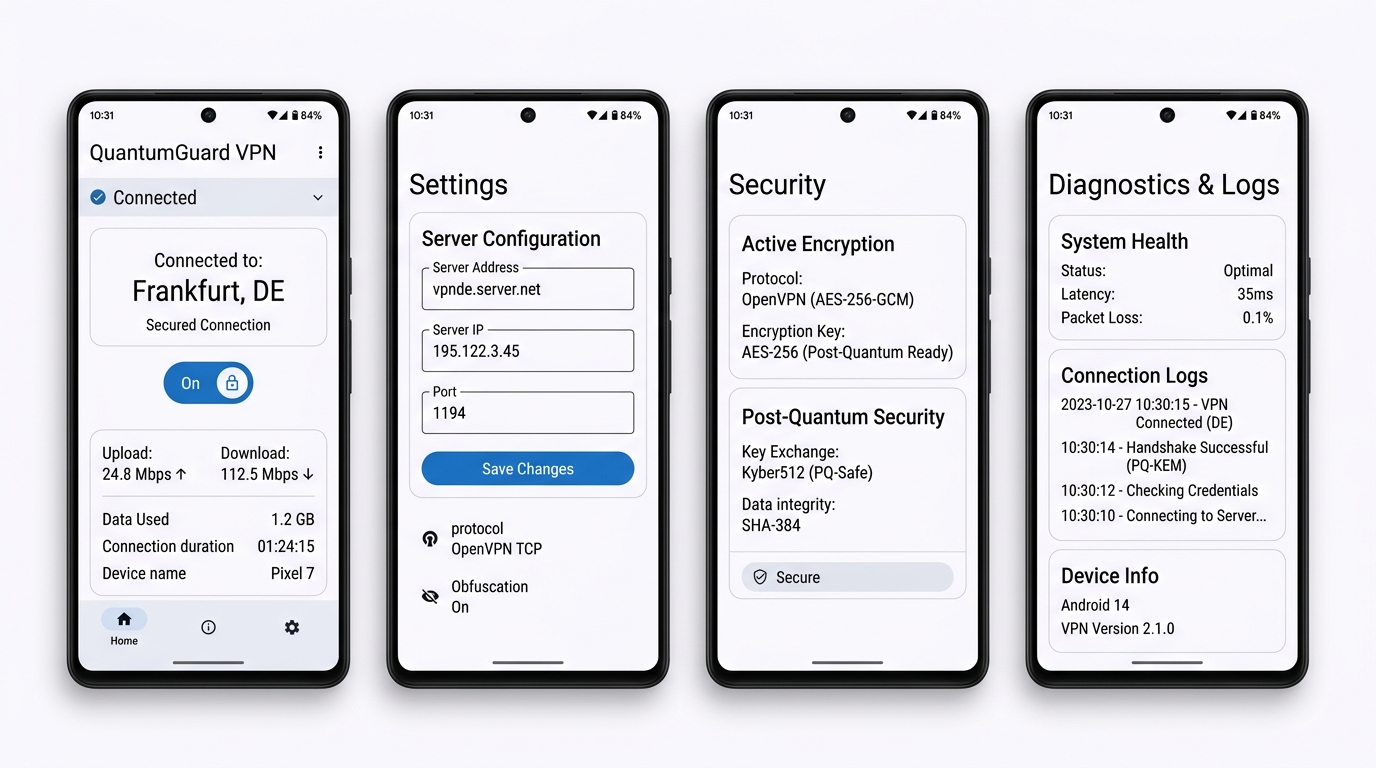
\includegraphics[width=0.82\linewidth,height=0.20\textheight,keepaspectratio]{figures/ui_screens_overview.jpg}
  \caption[Four-Screen Minimal White Design System Showcase]{Minimal White Design System Showcase: This figure illustrates the four core Android client screens comprising the Home Dashboard, Server Configuration, Cryptographic Information, and Diagnostic Terminal.}
  \label{fig:ui_screens_mockup}
\end{figure}

\subsection{Design System Tokens: Colors and Typography}
To enforce design consistency across the Kotlin Jetpack Compose codebase, the application implements a centralized token system within \texttt{ui/theme/Theme.kt} (Table~\ref{tab:design_tokens_color}). The typography scale leverages Google's Inter for headings and UI controls, paired with Roboto Mono for cryptographic hashes, IP addresses, and diagnostic logs. Spatial layout adheres to an 8-point grid: 16\,dp horizontal screen padding, 12\,dp component spacing, 12\,dp card corner radii, and 56\,dp primary button height with 0\,dp elevation shadows.

\begin{table}[htbp]
  \centering
  \scriptsize
  \setlength{\tabcolsep}{3pt}
  \caption{Design System Tokens: Color Palette and Semantic Usage.}
  \label{tab:design_tokens_color}
  \begin{tabularx}{\linewidth}{@{}p{2.8cm}p{1.4cm}p{1.8cm}Y@{}}
    \toprule
    \textbf{Design Token} & \textbf{Hex} & \textbf{Visual} & \textbf{Semantic Application} \\
    \midrule
    Surface Pure White & \texttt{\#FFFFFF} & Pure White & Primary background surface for all screens and cards \\
    Surface Container & \texttt{\#F8F9FA} & Ultra-Light Gray & Contrast surface for nested telemetry containers \\
    Border Structural & \texttt{\#DEE2E6} & Light Neutral & 1\,dp structural dividers and card outlines \\
    Text High Contrast & \texttt{\#1A1D20} & Dark Charcoal & Primary typography, titles, and status headlines \\
    Text Secondary & \texttt{\#6C757D} & Medium Gray & Metadata labels, subtitles, and unit indicators \\
    Brand Primary Blue & \texttt{\#1971C2} & Marine Blue & Primary interactive button (Connect), active tabs \\
    Brand Accent Light & \texttt{\#E7F5FF} & Ice Blue Tint & Status badge container for active connection \\
    Status Success Green & \texttt{\#2B8A3E} & Forest Green & Connected state indicator dot and success alerts \\
    Status Warning Amber & \texttt{\#E67700} & Deep Amber & Connecting / handshaking in-progress indicator \\
    Status Error Red & \texttt{\#C92A2A} & Crimson Red & Disconnection alerts, handshake failure badges \\
    \bottomrule
  \end{tabularx}
\end{table}

\subsection{Screen Architecture and Accessibility}
The mobile client deploys a single-activity architecture (\texttt{MainActivity.kt}) hosting four dedicated views:
\begin{enumerate}
    \item \textbf{Screen A (Home Dashboard):} Interactive pill-shaped connection badge, high-contrast session timer, primary action button, and live throughput cards.
    \item \textbf{Screen B (Server Configuration):} Outlined text fields with real-time regex validation for Server Hostname/IPv4, Port (7000), MTU (1400 bytes), and Socket Timeout.
    \item \textbf{Screen C (Cryptographic Security Info):} Transparency cards detailing ML-KEM-1024, ML-DSA-65, AES-256-GCM AEAD, and 64-bit anti-replay parameters.
    \item \textbf{Screen D (Diagnostics and Settings):} Operational kill-switch toggles, live diagnostic terminal, ping verification, and DNS leak tests.
\end{enumerate}
Accessibility compliance satisfies WCAG 2.1 AAA: dark charcoal text against pure white provides a 16.8:1 contrast ratio; touch targets enforce $48 \times 48$\,dp minimums; and every composable specifies semantic \texttt{contentDescription} attributes.

Figure~\ref{fig:tikz_uml_class} depicts the object-oriented structure of the Android client application adhering to the Model-View-ViewModel (MVVM) architectural pattern.

\begin{figure}[htbp]
  \centering
  \begin{tikzpicture}[
    scale=0.80, every node/.style={transform shape},
    classbox/.style={draw=darkcharcoal, thick, fill=white, rounded corners=2pt, align=left, font=\scriptsize}
  ]
    \node[classbox, minimum width=5.5cm] (vm) at (0, 3.8) {
      \textbf{\large VpnViewModel}\\
      \rule{5.4cm}{0.4pt}\\
      - \texttt{\_uiState: MutableStateFlow<VpnUiState>}\\
      - \texttt{\_telemetry: MutableStateFlow<TelemetryData>}\\
      \rule{5.4cm}{0.4pt}\\
      + \texttt{connect(host: String, port: Int): Unit}\\
      + \texttt{disconnect(): Unit}
    };

    \node[classbox, minimum width=6.2cm] (vpn) at (0, -0.8) {
      \textbf{\large QuantumSafeVpnService}\\
      \rule{6.1cm}{0.4pt}\\
      - \texttt{vpnInterface: ParcelFileDescriptor?}\\
      - \texttt{socketChannel: SocketChannel?}\\
      - \texttt{pqcEngine: PqcEngine}\\
      \rule{6.1cm}{0.4pt}\\
      + \texttt{onStartCommand(intent: Intent, ...): Int}\\
      + \texttt{connectVpn(host: String, port: Int, ...): Unit}
    };

    \node[classbox, minimum width=5.6cm] (pqc) at (7.2, -0.8) {
      \textbf{\large PqcEngine}\\
      \rule{5.5cm}{0.4pt}\\
      - \texttt{sessionKey: ByteArray?}\\
      \rule{5.5cm}{0.4pt}\\
      + \texttt{generateKemKeyPair(): KemKeyPair}\\
      + \texttt{decapsulateKem(sk: ByteArray, c: ByteArray): ByteArray}\\
      + \texttt{encryptAesGcm(key: ByteArray, p: ByteArray, s: Long): ByteArray}
    };

    \draw[thick, ->] (vm.south) -- node[right, font=\tiny\bfseries] {binds \& controls} (vpn.north);
    \draw[thick, ->] (vpn.east) -- node[above, font=\tiny\bfseries] {delegates crypto} (pqc.west);
  \end{tikzpicture}
  \caption[UML Class Hierarchy of Android Client Architecture]{UML Class Hierarchy: This figure illustrates the object-oriented architecture and reactive MVVM component relationships between VpnViewModel, QuantumSafeVpnService, and PqcEngine.}
  \label{fig:tikz_uml_class}
\end{figure}
